\chapter{Perancangan}
\label{chapter:perancangan}
Pada bab ini dibahas mengenai perancangan perangkat lunak yang meliputi: perancangan struktur web, perancangan antarmuka, dan perancangan fitur yang diimplementasikan pada Aplikasi Pratinjau 3 Dimensi Berbasis.

\section{Perancangan Struktur Web}
\label{sec:analisisStrukturWeb}

Struktur web merupakan susunan direktori yang membangun web tersebut. Struktur web terdiri dari berbagai folder dan berkas yang telah dipisahkan berdasarkan fungsinya masing-masing. Berikut ini merupakan penjelasan masing-masing folder dan berkas yang digunakan untuk membangun web ini:

\begin{itemize}
	\item {\bf folder css}, folder ini berisi berkas dengan ekstensi css yang digunakan untuk mengatur dan memperindah tampilan web. Berkas yang ada pada folder ini hanya satu yaitu custom.css.
	\item {\bf folder img}, folder ini berisi berkas gambar dengan ekstensi jpg. Terdapat berkas-berkas gambar seperti pilihan tekstur warna cat dinding dan pilihan tekstur warna lantai. Berikut ini merupakan daftar berkas yang ada pada folder ini:
	\begin{itemize}
		\item textureatap.jpg, merupakan tekstur untuk bagian atap ruangan kelas.
		\item texturedinding1.jpg, merupakan pilihan tekstur pertama untuk bagian dinding ruangan kelas.
		\item texturedinding2.jpg, merupakan pilihan tekstur kedua untuk bagian dinding ruangan kelas.
		\item texturedinding3.jpg, merupakan pilihan tekstur ketiga untuk bagian dinding ruangan kelas.
		\item texturedinding4.jpg, merupakan pilihan tekstur keempat untuk bagian dinding ruangan kelas.
		\item texturedinding5.jpg, merupakan pilihan tekstur kelima untuk bagian dinding ruangan kelas.
		\item texturedinding6.jpg, merupakan pilihan tekstur keenam untuk bagian dinding ruangan kelas.
		\item texturedinding7.jpg, merupakan pilihan tekstur ketujuh untuk bagian dinding ruangan kelas.
		\item texturedinding8.jpg, merupakan pilihan tekstur kedelapan untuk bagian dinding ruangan kelas.
		\item texturelantai1.jpg, merupakan pilihan tekstur pertama untuk bagian lantai ruangan kelas.
		\item texturelantai2.jpg, merupakan pilihan tekstur kedua untuk bagian lantai ruangan kelas.
		\item texturelantai3.jpg, merupakan pilihan tekstur ketiga untuk bagian lantai ruangan kelas.
		\item texturelantai4.jpg, merupakan pilihan tekstur keempat untuk bagian lantai ruangan kelas.
		\item texturelantai5.jpg, merupakan pilhan tekstur kelima untuk bagian lantai ruangan kelas.
		\item texturelantai6.jpg, merupakan pilihan teksur keenam untuk bagian lantai ruangan kelas.
		\item texturelantai7.jpg, merupakan pilihan tekstur ketujuh untuk bagian lantai ruangan kelas.
		\item texturelantai8.jpg, merupakan pilihan tekstur kedelapan untuk bagian lantai ruangan kelas.
	\end{itemize}
	\item {\bf folder js}, folder ini berisi berkas dengan ekstensi js. Terdapat berbagai file JavaScript di dalam folder ini, daftar berkasnya adalah sebagai berikut:
		\begin{itemize}
			\item {\bf Main.js}, berkas JavaScript ini berisi berbagai fungsi utama yang digunakan untuk membangun Aplikasi Pratinjau 3 Dimensi Berbasis Web.
			\item {\bf three.js}, berkas JavaScript ini berisi berbagai fungsi yang disediakan oleh pustaka Three.js. Nantinya fungsi yang terdapat di dalam berkas ini akan dipanggil oleh Main.js
			\item {\bf OrbitControls.js}, berkas JavaScript ini berisi berbagai fungsi yang juga disediakan oleh pustaka Three.js. Namun pada berkas ini hanya khusus menyediakan fungsi-fungsi yang berkaitan dengan kontrol pada kamera.
		\end{itemize}
	\item {\bf folder json}, folder ini berisi berkas dengan ekstensi JSON. Terdapat 2 berkas json di dalam folder ini yaitu sebagai berikut:
		\begin{itemize}
			\item {\bf constant.json}, berkas ini berisi berbagai informasi awal untuk diinisialisasi ke aplikasi sehingga dapat menampilkan gambaran awal dari ruangan kelas Fakultas Teknologi Informasi dan Sains.
			\item {\bf imported.json}, berkas ini berisi informasi untuk repsentasi ruangan kelas saat ujian sedang berlangsung di Fakultas Teknologi Informasi dan Sains.
		\end{itemize}
	\item {\bf folder models}, folder ini berisi semua berkas yang diperlukan untuk membuat semua model pada Aplikasi Pratinjau 3 Dimensi Berbasis Web dengan ekstensi JSON (JavaScript Object Notation) dan ekstensi jpg. Berikut ini merupakan daftar berkas yang terdapat pada folder ini:
	\begin{itemize}
		\item Berkas dengan ekstensi JSON. Berkas ini berisi semua nilai informasi yang merepresentasikan suatu model seperti material yang digunakan serta koordinat titik-titik yang membentuk model tersebut. Daftar berkas dengan ekstensi JSON adalah sebagai berikut:
		\begin{itemize}
			\item ac.json, berkas yang berisi nilai informasi untuk model {\it air conditioner} pada ruangan kelas.
			\item jamdinding.json, berkas yang berisi nilai informasi untuk model jam dinding pada ruangan kelas.
			\item jendela.json, berkas yang berisi nilai informasi untuk model jendela pada ruangan kelas.
			\item kursidosen.json, berkas yang berisi nilai informasi untuk model kursi dosen pada ruangan kelas.
			\item kursimahasiswa.json, berkas yang berisi nilai informasi untuk model kursi mahasiswa pada ruangan kelas.
			\item lampu.json, berkas yang berisi nilai informasi untuk model lampu pada ruangan kelas.
			\item layar.json, berkas yang berisi nilai informasi untuk model layar proyektor pada ruangan kelas.
			\item mejadosen.json, berkas yang berisi nilai informasi untuk model meja dosen pada ruangan kelas.
			\item papantulis.json, berkas yang berisi nilai informasi untuk model papan tulis pada ruangan kelas.
			\item pintu.json, berkas yang berisi nilai informasi untuk model pintu pada ruangan kelas.
			\item proyektor.json, berkas yang berisi nilai informasi untuk model proyektor pada ruangan kelas.
		\end{itemize}
		\item Berkas dengan ekstensi jpg. Berkas ini berisi tekstur gambar yang akan dipetakan ke model dengan ekstensi JSON yang telah dibahas sebelumnya. Daftar berkas dengan ekstensi jpg pada folder ini adalah sebagai berikut:
		\begin{itemize}
			\item textureacproyektorlayar.jpg, merupakan tekstur yang akan dipetakan ke model {\it air conditioner}, proyektor, dan layar.
			\item texturejamdinding, merupakan tekstur yang akan dipetakan ke model jam dinding.
			\item texturejendela.jpg, merupakan tekstur yang akan dipetakan ke model jendela.
			\item texturekursidosen.jpg, merupakan tekstur yang akan dipetakan ke model kursi dosen.
			\item texturekursimahasiswa.jpg, merupakan tekstur yang akan dipetakan ke model kursi mahasiswa.
			\item texturelampu.jpg, merupakan tekstur yang akan dipetakan ke model lampu.
			\item texturemejadosen.jpg, merupakan tekstur yang akan dipetakan ke model meja dosen.
			\item texturepapantulis.jpg, merupakan tekstur yang akan dipetakan ke model papan tulis.
			\item texturepintu.jpg, merupakan tekstur yang akan dipetakan ke model pintu.
		\end{itemize} 
	\end{itemize}
	\item {\bf berkas index.html}, merupakan berkas {\it HyperText Markup Language} (HTML) yang membentuk web untuk aplikasi pratinjau ini.
\end{itemize}

\section{Perancangan Antarmuka}
\label{sec:perancanganAntarmuka}
Perancangan antarmuka dibuat atas dasar kebutuhan pengguna dengan Aplikasi Pratinjau 3 Dimensi Berbasis Web. Antarmuka ini digunakan sebagai media komunikasi antara pengguna dengan aplikasi web yang dibangun. Antarmuka untuk aplikasi ini terbagi menjadi dua jendela utama yaitu antarmuka masukkan dan antarmuka keluaran seperti pada gambar ~\ref{fig:antarmuka1}. Berikut ini merupakan rancangan antarmuka aplikasi yang akan dibangun:
\begin{figure}[ht]
	\centering
	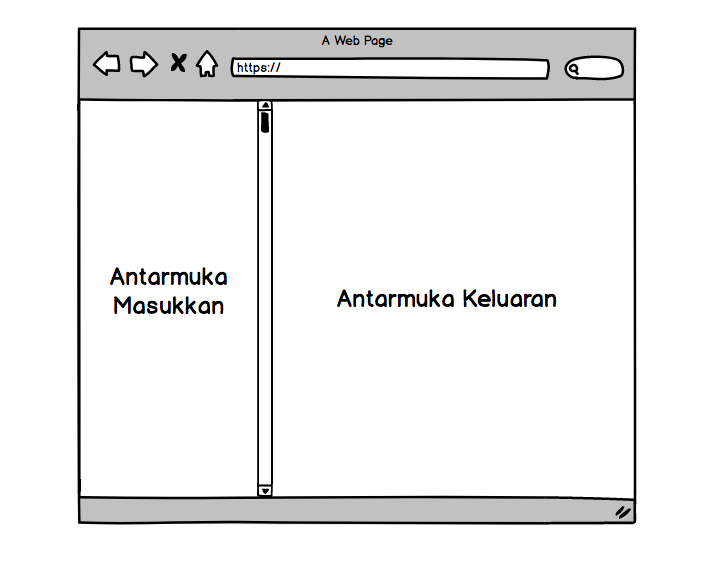
\includegraphics[scale=0.3]{antarmuka1}
	\caption{Rancangan antarmuka secara keseluruhan.}
	\label{fig:antarmuka1}
	\vspace{8mm}
\end{figure}

\subsection{Rancangan Antarmuka Masukkan}
\label{sec:antarmukamasukkan}
Melalui antarmuka ini pengguna dapat memberikan masukkan untuk mengubah kondisi kelas yang sedang dipratinjau. Rancangan untuk antarmuka ini dapat dilihat pada gambar ~\ref{fig:antarmuka2}. Penjelasan untuk setiap masukkan pada gambar tersebut akan dijelaskan berikut ini:
\begin{itemize}
	\item Pilihan, merupakan pilihan yang dapat diambil untuk hasil pratinjau yang telah dibuat.
		\begin{itemize}
			\item Buat ulang desain, merupakan tombol yang berfungsi untuk memperbarui halaman web sehingga masukkan yang telah diberikan sebelumnya akan diabaikan dan dimulai ulang dari awal.
			\item {\it Print} hasil pratinjau, merupakan tombol yang berfungsi untuk mencetak hasil pratinjau.
		\end{itemize}
	\item Mode pratinjau, merupakan pilihan untuk posisi untuk melihat pratinjau ruangan kelas.
		\begin{itemize}
			\item Dalam kelas, merupakan tombol untuk pilihan melihat pratinjau dari dalam ruangan kelas.
			\item Luar kelas, merupakan tombol untuk pilihan melihat pratinjau dari luar ruangan kelas.
		\end{itemize}
	\item Masukkan JSON, merupakan pilihan untuk memberikan masukkan properti ke dalam kelas dengan ekstensi {\it JavaScript Object Notation} (JSON) sesuai format yang telah disediakan.
	\item Warna dinding, merupakan varian warna dinding yang dapat dipilih oleh pengguna untuk mengubah warna dari dinding ruangan.
	\item Warna lantai, merupakan varian warna lantai yang dapat dipilih oleh pengguna untuk mengubah warna dari lantai ruangan.
\end{itemize}
\begin{figure}[ht]
	\centering
	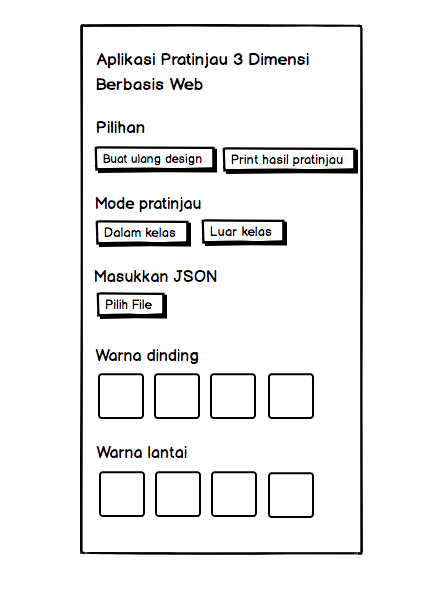
\includegraphics[scale=0.5]{antarmuka2}
	\caption{Rancangan antarmuka masukkan.}
	\label{fig:antarmuka2}
	\vspace{8mm}
\end{figure}

\subsection{Rancangan Antarmuka Keluaran}
\label{sec:antarmukakeluaran}
Melalui antarmuka ini pengguna dapat melihat kondisi kelas yang sedang dipratinjau. Pengguna dapat melakukan rotasi untuk melihat sisi lain dari ruangan kelas yang sedang dimodelkan pada antarmuka ini. Rancangan untuk antarmuka ini dapat dilihat pada gambar \ref{fig:antarmuka3}.
\begin{figure}[ht]
	\centering
	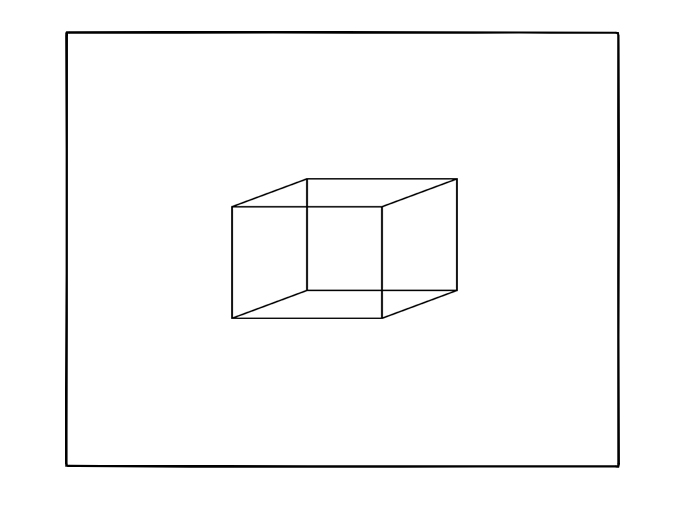
\includegraphics[scale=0.6]{antarmuka3}
	\caption{Rancangan antarmuka keluaran.}
	\label{fig:antarmuka3}
	\vspace{8mm}
\end{figure}

\section{Rancangan Fitur yang Akan Diimplementasikan}
\label{sec:rancanganfitur}
Terdapat beberapa fitur yang akan diimplementasikan untuk Aplikasi Pratinjau 3 Dimensi. Fitur-fitur tersebut dibuat untuk mendukung kegiatan pengguna dalam merasakan proses dan hasil pratinjau yang lebih baik. Berikut ini merupakan penjelasan untuk fitur-fitur tersebut:

\subsection{Fitur Mengganti Warna Dinding dan Warna Lantai Ruangan Kelas}
\label{sec:fiturgantiwarna}
Fitur ini berguna untuk mengganti warna tekstur dinding dan warna tekstur lantai yang sesuai dengan keinginan pengguna. Pengguna akan memilih warna tekstur dinding dan tekstur lantai pada pilihan masukkan di bagian kiri layar. Kemudian setelah itu hasil pilihan warna tekstur yang dipilih pengguna akan teraplikasikan pada model ruangan kelas di bagian kanan layar. Contoh gambar untuk pengguna yang memilih warna merah jambu untuk warna tekstur dinding dan abu-abu untuk warna tekstur lantai dapat dilihat pada gambar ~\ref{fig:antarmuka4}.
\begin{figure}[ht]
	\centering
	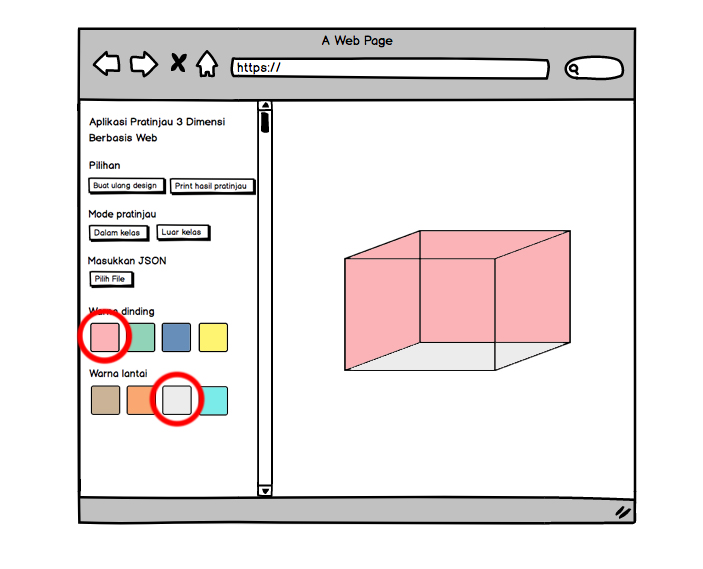
\includegraphics[scale=0.6]{antarmuka4}
	\caption{Fitur mengganti warna dinding dan lantai.}
	\label{fig:antarmuka4}
	\vspace{8mm}
\end{figure}

\subsection{Fitur Unggah berkas JSON untuk Menambah dan Mengganti Isi Informasi Ruangan Kelas}
\label{sec:fiturunggahjson}
Fitur ini berguna untuk menambahkan dan mengganti isi informasi ruangan kelas. Informasi seperti properti ruangan kelas dapat ditambah dan diganti dengan mengunggah berkas dengan ekstensi JSON pada pilihan masukkan di bagian kiri. Berkas JSON untuk beberapa mode kelas seperti saat sedang kegiatan perkuliahan, kegiatan ujian, maupun keadaan kelas yang kosong telah disediakan pada folder json. Pengguna dapat mengubah isi JSON tersebut dan menggunggah kembali untuk merubah keadaan ruangan kelas sesuai dengan yang pengguna inginkan. Contoh JSON untuk properti kelas pada saat kegiatan ujian dapat dilihat pada {\it listing} ~\ref{lst:json}.
\begin{lstlisting}[caption={Contoh JSON untuk ruangan kelas pada saat ujian.}, label={lst:json},captionpos=b]
var constant = {
        "worldColor": 0xa9d9ef,
        "control": {
            "minZoom": 15,
            "maxZoom": 42
        },
        "classProperties": [
        {
            "dx": 19.5,
            "dy": 4,
            "dz": 14.2,
            "distancex": -3,
            "distancez": -3.5,
            "repeatx": 6,
            "repeaty": 5,
            "rotation": 0,
            "texture": "models/texturekursimahasiswa.jpg",
            "model": "models/kursimahasiswa.json",
            "scale": 1
        },{
            "dx": -4,
            "dy": 4,
            "dz": 14.2,
            "distancex": -3,
            "distancez": -3.5,
            "repeatx": 6,
            "repeaty": 5,
            "rotation": 0,
            "texture": "models/texturekursimahasiswa.jpg",
            "model": "models/kursimahasiswa.json",
            "scale": 1
        },
            {
                "dx": 19.5,
                "dy": 10.2,
                "dz": 17.1,
                "distancex": -3,
                "distancez": 0,
                "repeatx": 14,
                "repeaty": 1,
                "rotation": 3.14159,
                "texture": "models/texturejendela.jpg",
                "model": "models/jendela.json",
                "scale": 2
            },
            {
                "dx": 8,
                "dy": 4.7,
                "dz": -8,
                "distancex": 6,
                "distancez": 0,
                "repeatx": 2,
                "repeaty": 1,
                "rotation": Math.PI + (Math.PI/2),
                "texture": "models/texturemejadosen.jpg",
                "model": "models/mejadosen.json",
                "scale": 2
            },
            {
                "dx": -8,
                "dy": 14.5,
                "dz": -14.9,
                "distancex": 13,
                "distancez": 0,
                "repeatx": 2,
                "repeaty": 1,
                "rotation": 0,
                "texture": "models/textureacproyektorlayar.jpg",
                "model": "models/layar.json",
                "scale": 1
            },
            {
                "dx": -4,
                "dy": 14,
                "dz": 0,
                "distancex": 13,
                "distancez": 0,
                "repeatx": 2,
                "repeaty": 1,
                "rotation": Math.PI,
                "texture": "models/textureacproyektorlayar.jpg",
                "model": "models/proyektor.json",
                "scale": 1
            },
            {
                "dx": -15,
                "dy": 13,
                "dz": 14.5,
                "distancex": 15,
                "distancez": 0,
                "repeatx": 3,
                "repeaty": 1,
                "rotation": Math.PI,
                "texture": "models/textureacproyektorlayar.jpg",
                "model": "models/ac.json",
                "scale": 1
            },
            {
                "dx": -13,
                "dy": 14.9,
                "dz": -5,
                "distancex": 10,
                "distancez": 10,
                "repeatx": 3,
                "repeaty": 2,
                "rotation": 0,
                "texture": "models/texturelampu.jpg",
                "model": "models/lampu.json",
                "scale": 1
            },
            {
                "dx": 2.7,
                "dy": 14,
                "dz": -15.2,
                "distancex": 0,
                "distancez": 0,
                "repeatx": 1,
                "repeaty": 1,
                "rotation": 0,
                "texture": "models/texturejamdinding.jpg",
                "model": "models/jamdinding.json",
                "scale": 1
            },
            {
                "dx": -13,
                "dy": 7.5,
                "dz": -14.6,
                "distancex": 0,
                "distancez": 0,
                "repeatx": 1,
                "repeaty": 1,
                "rotation": 0,
                "texture": "models/texturepintu.jpg",
                "model": "models/pintu.json",
                "scale": 2
            },
            {
                "dx": 10,
                "dy": 5.5,
                "dz": -12,
                "distancex": 0,
                "distancez": 0,
                "repeatx": 1,
                "repeaty": 1,
                "rotation": 0,
                "texture": "models/texturekursidosen.jpg",
                "model": "models/kursidosen.json",
                "scale": 1.5
            }
        ],
        "room": {
            "texture": {
                "wall": [
                    "img/texturedinding1.jpg",
                    "img/texturedinding2.jpg",
                    "img/texturedinding3.jpg",
                    "img/texturedinding4.jpg",
                    "img/texturedinding5.jpg",
                    "img/texturedinding6.jpg",
                    "img/texturedinding7.jpg",
                    "img/texturedinding8.jpg"
                ],
                "floor": [
                    "img/texturelantai1.jpg",
                    "img/texturelantai2.jpg",
                    "img/texturelantai3.jpg",
                    "img/texturelantai4.jpg",
                    "img/texturelantai5.jpg",
                    "img/texturelantai6.jpg",
                    "img/texturelantai7.jpg",
                    "img/texturelantai8.jpg"
                ],
                "ceiling": "img/textureatap.jpg"
            },
            "size": {
                "length": 43,
                "width": 12,
                "height": 31
            }
        },
        "view": {
            "outside": {
                "cameraPosition": {
                    "x": 0,
                    "y": 10,
                    "z": 40
                },
                "control": {
                    "minZoom": 10,
                    "maxZoom": 42
                },
                "target": {
                    "x": 0,
                    "y": 10,
                    "z": 0
                }
            },
            "inside": {
                "cameraPosition": {
                    "x": 0,
                    "y": 10,
                    "z": 0
                },
                "control": {
                    "minZoom": 5,
                    "maxZoom": 15
                },
                "target": {
                    "x": 0,
                    "y": 10,
                    "z": 0
                }
            },
            "init": {
                "verticalField": 75,
                "nearPlane": 0.1,
                "farPlane": 100
            }
        } 
    }
\end{lstlisting}

Berikut ini merupakan penjelasan untuk setiap isi objek pada JSON tersebut:
\begin{itemize}
	\item {\it worldColor}, merupakan warna latar dari ruang tempat dilakukannya pemodelan kelas.
	\item {\it control}, merupakan ukuran perbesaran kamera minimal dan maksimal yang dibagi menjadi objek {\it minZoom} dan {\it maxZoom}.
	\item {\it classProperties}, merupakan {\it array} dari objek-objek properti yang ada di dalam ruangan kelas. Terdapat beberapa objek lagi di dalamnya dengan penjelasan sebagai berikut:
	\begin{itemize}
		\item dx, merupakan posisi pada sumbu X dari suatu properti.
		\item dy, merupakan posisi pada sumbu Y dari suatu properti.
		\item dz, merupakan posisi pada sumbu Z dari suatu properti.
		\item distancex, merupakan jarak antara properti yang sama pada sumbu X apabila terdapat lebih dari satu properti yang sama.
		\item distancez, merupakan jarak antara properti yang sama pada sumbu Z apabila terdapat lebih dari satu properti yang sama. 
		\item repeatx, merupakan jumlah properti yang ingin dimunculkan pada arah sumbu X.
		\item repeatz, merupakan jumlah properti yang ingin dimunculkan pada arah sumbu Z.
		\item rotation, merupakan derajat rotasi dalam phi.
		\item texture, merupakan alamat berkas tekstur yang ingin dipetakan pada properti tersebut.
		\item model, merupakan alamat berkas model untuk properti tersebut.
		\item scale, merupakan kelipatan perbesaran yang ingin dilakukan pada properti apabila properti dirasa kurang proposional pada ruangan kelas.
	\end{itemize}
	\item room, merupakan objek yang berisi informasi ruangan kelas. Terdapat beberapa objek lagi di dalamnya dengan penjelasan sebagai berikut:
		\begin{itemize}
			\item texture, berisi pilihan tekstur untuk diaplikasikan pada ruangan kelas. Berikut ini penjelasan masing-masing objek di dalamnya:
			\begin{itemize}
				\item wall, merupakan {\it array} dari alamat-alamat berkas pilihan tekstur untuk dinding ruangan kelas.
				\item floor, merupakan {\it array} dari alamat-alamat berkas pilihan tekstur untuk lantai ruangan kelas.
				\item ceiling, merupakan alamat berkas tekstur untuk langit-langit ruangan kelas.
			\end{itemize}
			\item size, merupakan ukuran panjang, lebar, dan tinggi ruangan kelas yang dibagi menjadi objek {\it length, width,} dan {\it height}.
		\end{itemize}
	\item view, merupakan objek yang berisi pengaturan perspektif kamera dengan berbagai mode. Terdapat beberapa objek untuk representasi masing-masing mode yang akan dijelaskan berikut ini:
		\begin{itemize}
			\item outside, merupakan objek untuk mode kamera saat berada di luar ruangan kelas. Berikut ini masing-masing penjelasan informasi objek yang ada pada mode ini:
			\begin{itemize}
				\item cameraPosition, merupakan posisi kamera pada setiap sumbu yang terbagi menjadi objek x, y, dan z.
				\item control, merupakan nilai minimal dan maksimal jarak perbesaran yang dapat dilakukan kamera pada mode ini sehingga terbagi menjadi objek minZoom dan maxZoom.
				\item target, merupakan titik tempat kemera mengarah sehingga dibagi menjadi objek x, y, dan z.
			\end{itemize}
			\item inside, merupakan objek untuk mode kamera saat berada di dalam ruangan kelas. Berikut ini masing-masing penjelasan informasi objek yang ada pada mode ini:
			\begin{itemize}
				\item cameraPosition, merupakan posisi kamera pada setiap sumbu yang terbagi menjadi objek x, y, dan z.
				\item control, merupakan nilai minimal dan maksimal jarak perbesaran yang dapat dilakukan kamera pada mode ini sehingga terbagi menjadi objek minZoom dan maxZoom.
				\item target, merupakan titik tempat kemera mengarah sehingga dibagi menjadi objek x, y, dan z.
			\end{itemize}
			\item init, merupakan objek untuk inisialisasi awal kamera saat aplikasi ini dibuka. Berikut ini masing-masing penjelasan informasi objek yang ada pada mode ini:
			\begin{itemize}
				\item verticalField, merupakan nilai frustum pandang vertikal untuk kamera.
				\item nearPlane, merupakan nilai frustum jarak dekat untuk kamera.
				\item farPlane, merupakan nilai frustum jarak jauh untuk kamera.
			\end{itemize}
		\end{itemize}
\end{itemize}

\subsection{Fitur Halaman Web yang Responsif}
\label{sec:fiturcetakhasil}
Fitur ini berguna agar saat hasil pratinjau ruangan kelas Fakultas Teknologi Informasi dan Sains dicetak hasilnya dapat terlihat rapih. Web yang responsif akan membuat pemadatan antarmuka web ke kertas untuk cetak akan menjadi rapih dan tertata dengan baik. Pada pengimplementasiannya, fitur ini memanfaatkan fitur cetak bawaan dari peramban untuk mencetak halaman web. Sehingga melalui fitur ini, diharapkan pengguna dapat menggunakan hasil pratinjau tersebut untuk proses selanjutnya yang ingin dilakukan terhadap ruangan kelas Fakultas Teknologi Informasi dan Sains. Contoh implementasi fitur ini dapat dilihat pada gambar ~\ref{fig:print}.
\begin{figure}[!hb]
	\centering
	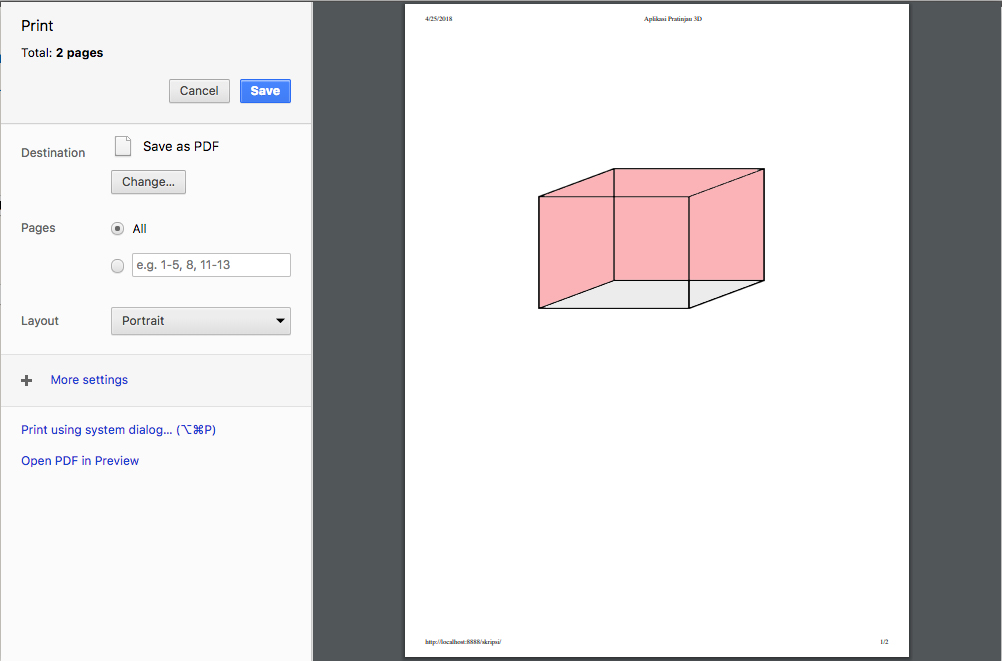
\includegraphics[scale=0.32]{print1}
	\caption{Fitur cetak pada peramban.}
	\label{fig:print}
	\vspace{8mm}
\end{figure}
















